\chapter{Resultados e Análise}
\label{cap:resultados}

\section{Calibração de \textit{M}}
\label{sec:res-calibracao}

A Figura \ref{fig:calib-tempo} apresenta o tempo mediano de execução em função de
$M$, e a Figura \ref{fig:calib-comp}, o número de comparações. A Tabela
\ref{tab:calibracao} resume os valores obtidos.

\begin{figure}[H]
\centering
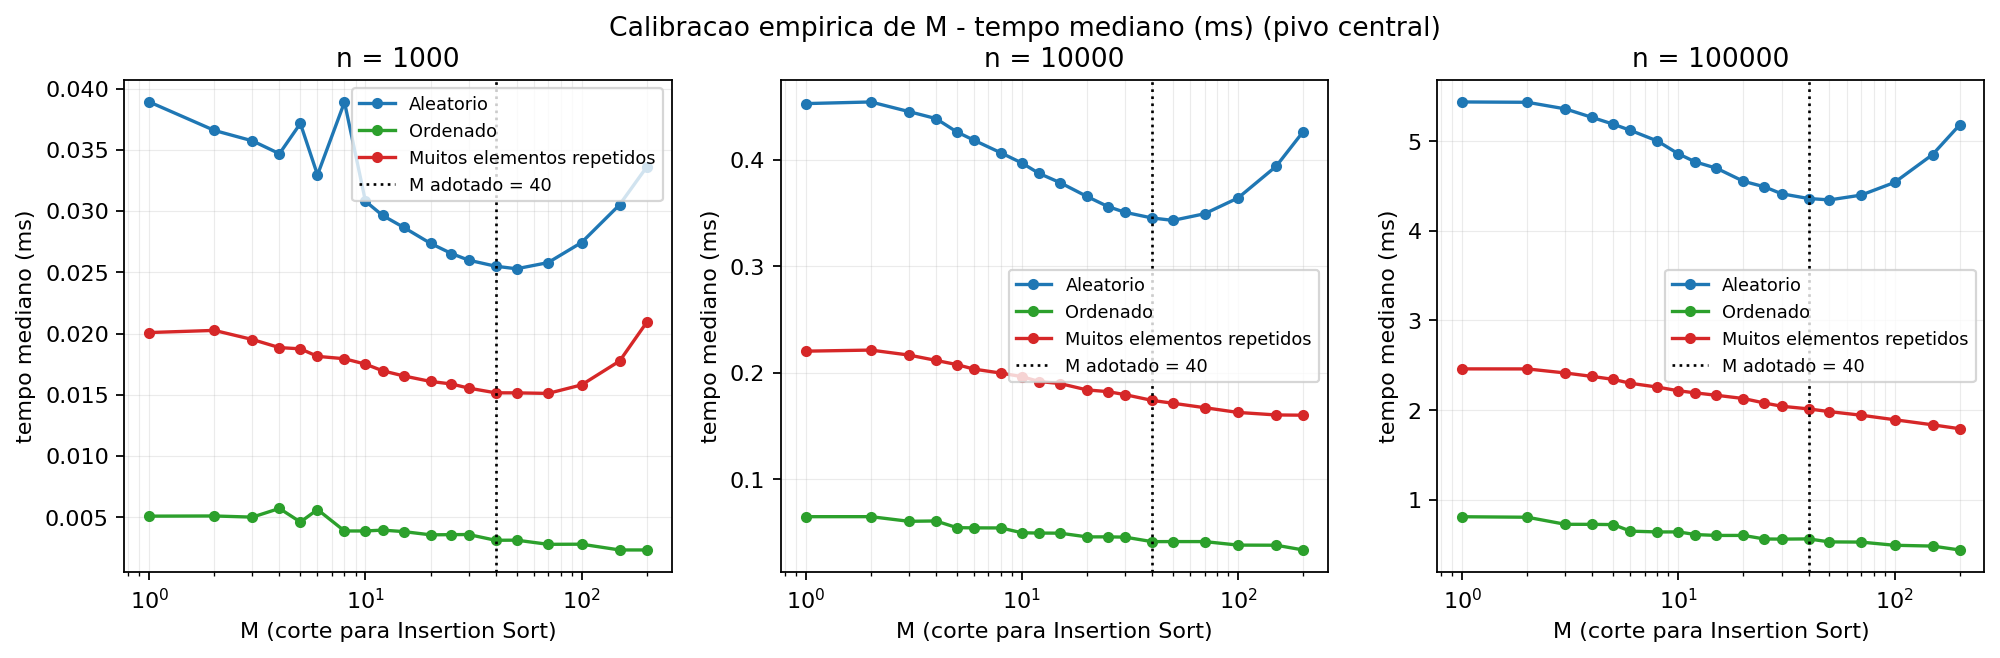
\includegraphics[width=\textwidth]{imagem/calibracao_m_tempo.png}
\caption{Tempo mediano de execução em função de $M$, para três tamanhos de entrada.}
\label{fig:calib-tempo}
\end{figure}
\FloatBarrier

\begin{figure}[H]
\centering
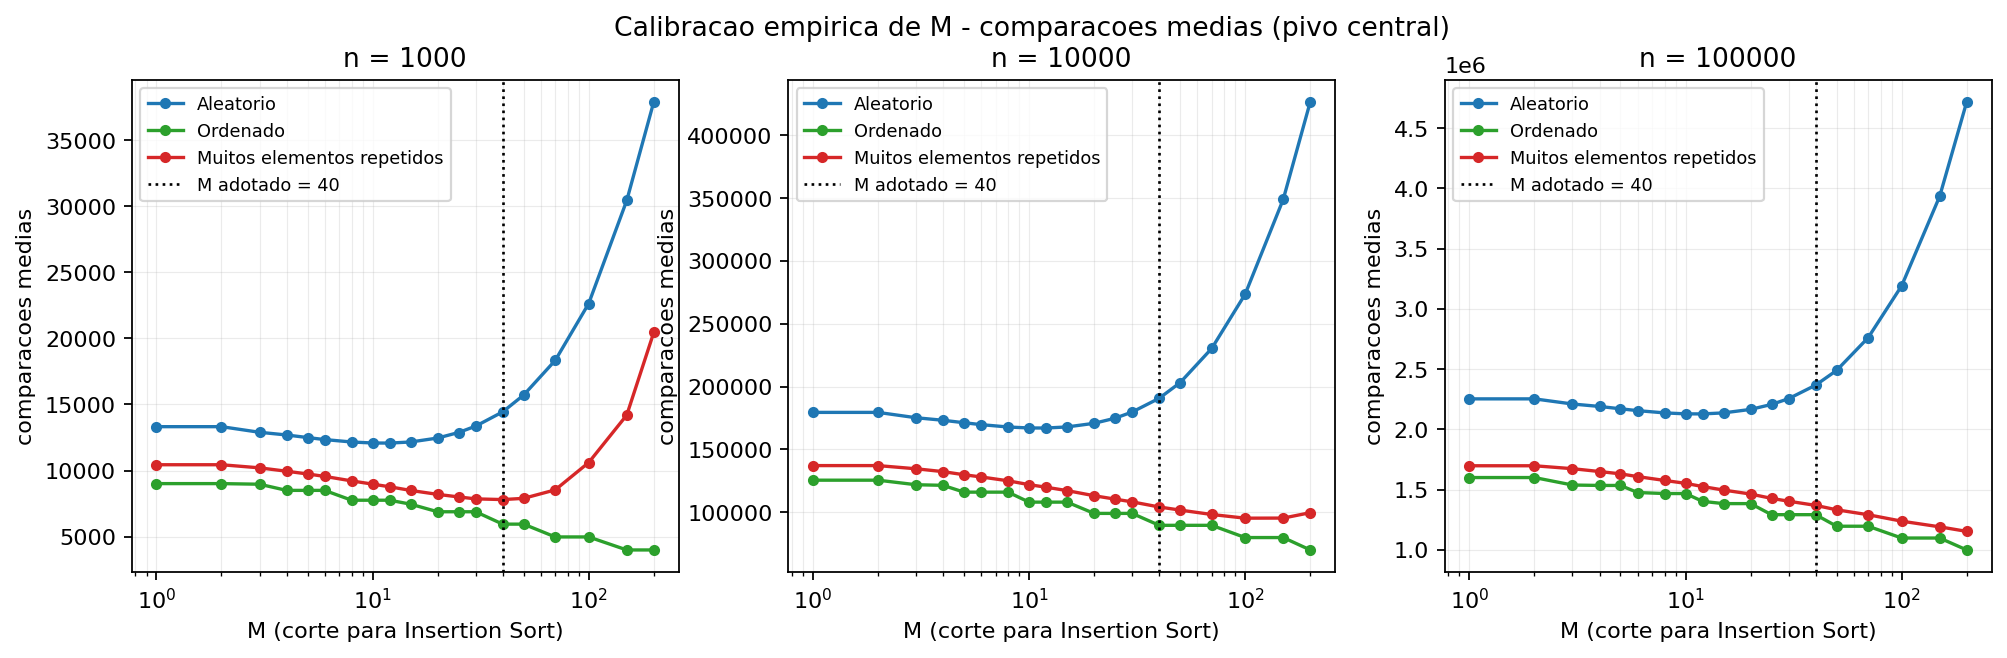
\includegraphics[width=\textwidth]{imagem/calibracao_m_comparacoes.png}
\caption{Número médio de comparações em função de $M$.}
\label{fig:calib-comp}
\end{figure}
\FloatBarrier

\begin{table}[H]
\centering
\caption{Valores de $M$ obtidos pela calibração empírica. A coluna ``$M$ recomendado'' usa o critério do menor $M$ dentro de 2\% do melhor tempo; a coluna ``$M$ por comparações'' usa o mínimo do número de comparações.}
\label{tab:calibracao}
\begin{tabular}{lccc}
\hline
\textbf{Estratégia de pivô} & \textbf{$n$} & \textbf{$M$ recomendado} & \textbf{$M$ por comparações} \\
\hline
Elemento central & 1.000 & 40 & 20 \\
Elemento central & 10.000 & 40 & 20 \\
Elemento central & 100.000 & 40 & 25 \\
Mediana de três & 1.000 & 40 & 20 \\
Mediana de três & 10.000 & 40 & 20 \\
Mediana de três & 100.000 & 40 & 25 \\
\hline
\end{tabular}
\end{table}

Três observações merecem destaque.

\paragraph{Estabilidade.} Os dois critérios comportam-se de forma distinta. O
\textbf{mínimo do número de comparações} --- métrica determinística, imune a ruído ---
é estável em $M \approx 20$--$25$ nas seis células. O \textbf{mínimo de tempo}
localiza-se em valores mais altos ($M \approx 50$--$70$) e seu \textit{argmin} exato
desloca-se conforme a célula, pois o platô é plano e a posição do mínimo passa a ser
determinada por ruído de medição. Por isso o critério adotado não é o \textit{argmin},
e sim o menor $M$ dentro de 2\% do melhor tempo, que conduz a $M = 40$ em
\textbf{todas as seis células}. Adotou-se $M = 40$ nos experimentos subsequentes por
ser o valor recomendado de forma unânime e por manter o Insertion Sort restrito a
subvetores pequenos.

\paragraph{Divergência entre os critérios.} O mínimo do número de comparações ocorre
em $M \approx 20$--$25$, enquanto o mínimo do tempo ocorre em valores mais altos. A
divergência é informativa: acima de $M = 25$, o algoritmo passa a executar
\textit{mais} comparações e ainda assim torna-se \textit{mais rápido}. Esse fenômeno
é analisado na Seção \ref{sec:analise-critica}. O platô de tempo (valores dentro de
2\% do melhor) estende-se, na maioria das células, de $M \approx 40$ a $M \approx 100$;
quem fica próximo de 20 é o mínimo de \textbf{comparações}, não o de tempo.

\paragraph{Comparação com a literatura.} O valor obtido é superior à faixa de 5 a 25
sugerida por \citeonline{sedgewick1978}. A diferença é coerente com a evolução do
hardware: as recomendações clássicas foram estabelecidas em máquinas nas quais o
custo relativo de uma comparação era muito maior que o de um acesso à memória. Em
processadores atuais, o Insertion Sort sobre blocos pequenos apresenta localidade de
cache e previsibilidade de desvios excelentes, além de ser passível de vetorização
pelo compilador, o que desloca o ponto de equilíbrio para valores maiores de $M$.
Soma-se a isso o fato de as chaves utilizadas serem do tipo \texttt{int}, cuja
movimentação é barata, favorecendo ainda mais o Insertion Sort.

\section{Comparação entre as três versões}

As Figuras \ref{fig:princ-tempo}, \ref{fig:princ-comp} e \ref{fig:princ-trocas}
apresentam, respectivamente, o tempo mediano, o número de comparações e o número de
trocas para as três versões, em escala logarítmica nos dois eixos. As Tabelas
\ref{tab:aleatorio} a \ref{tab:quaseordenado} trazem os valores numéricos.

\begin{figure}[H]
\centering
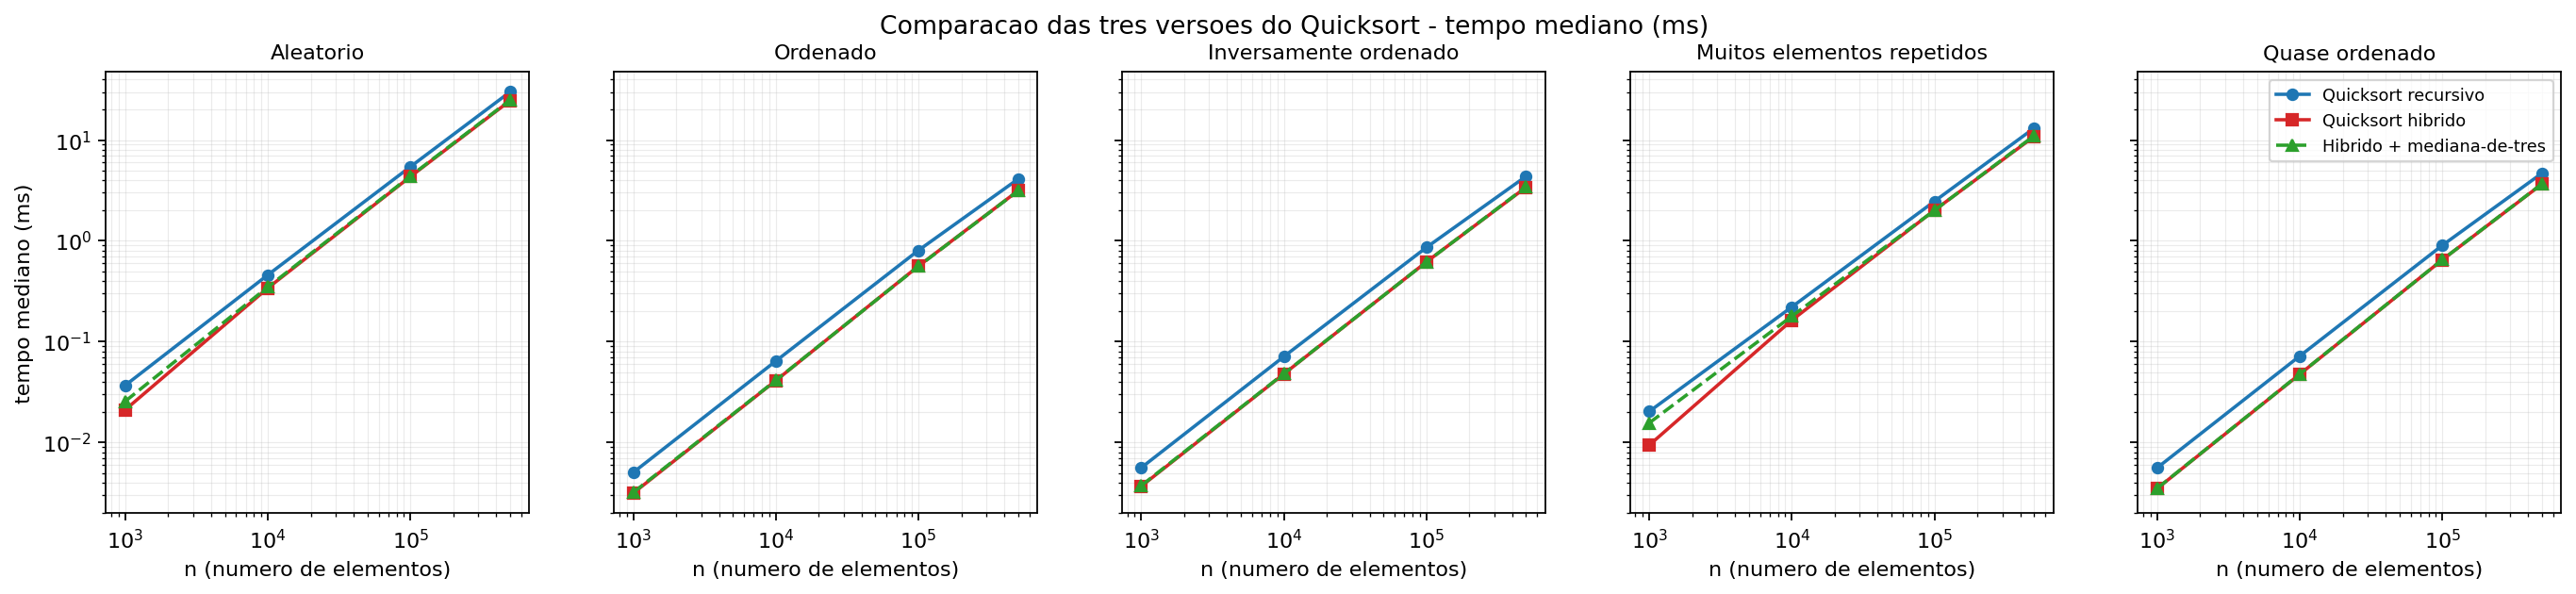
\includegraphics[width=\textwidth]{imagem/principal_tempo.png}
\caption{Tempo mediano de execução das três versões, por massa de teste.}
\label{fig:princ-tempo}
\end{figure}
\FloatBarrier

\begin{figure}[H]
\centering
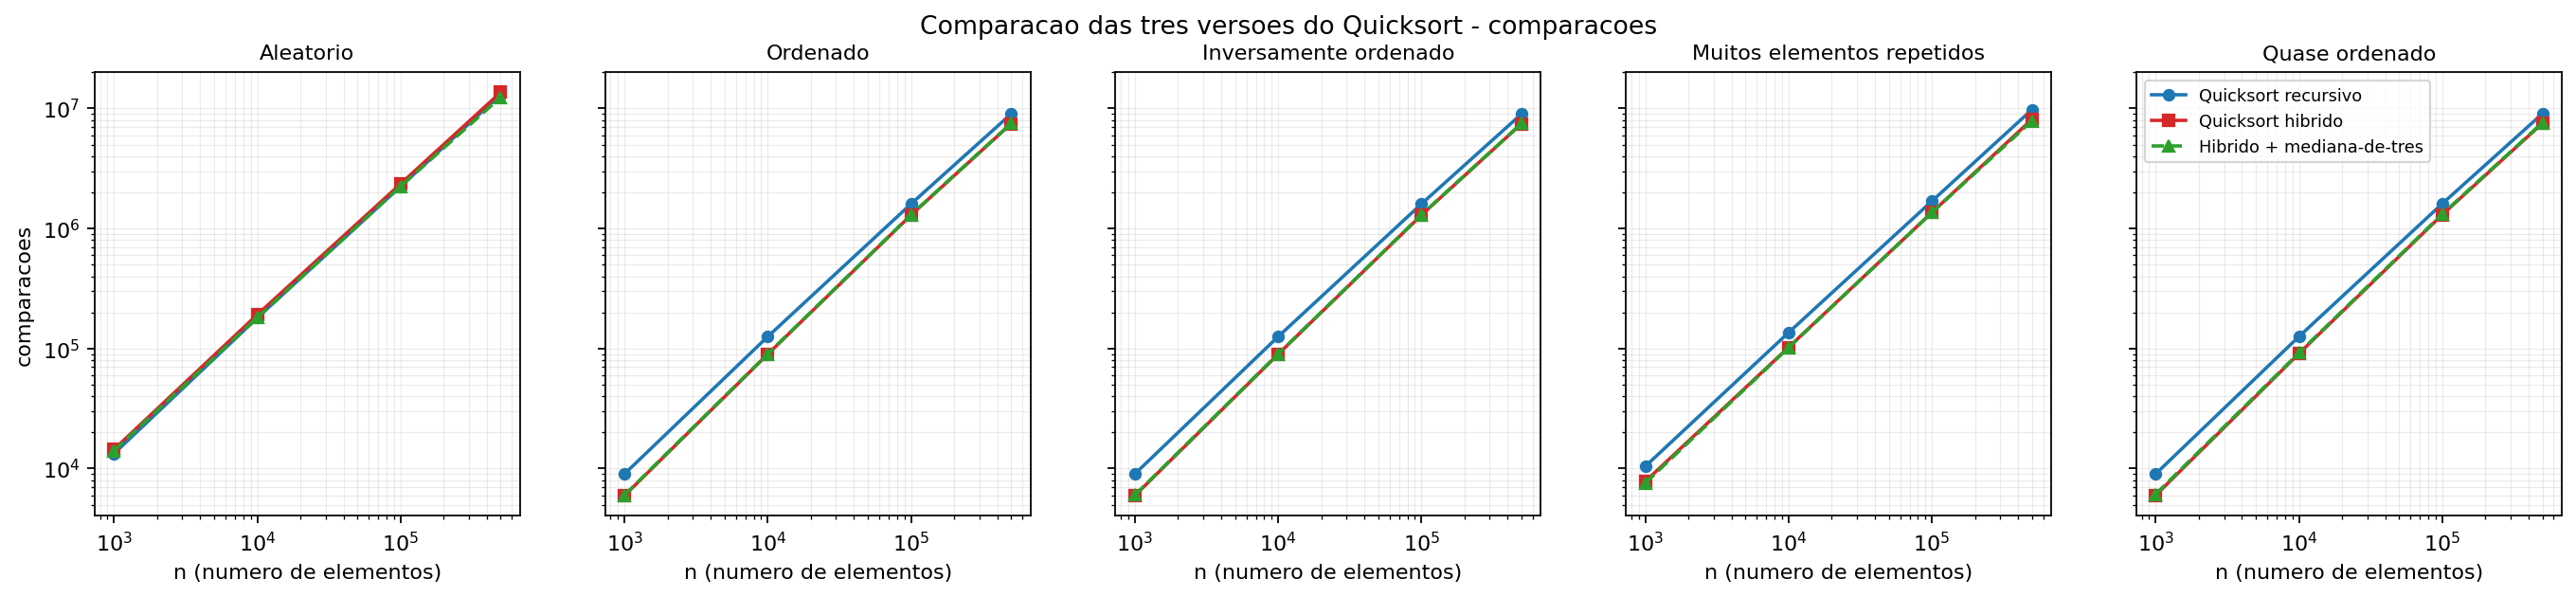
\includegraphics[width=\textwidth]{imagem/principal_comparacoes.png}
\caption{Número médio de comparações das três versões, por massa de teste.}
\label{fig:princ-comp}
\end{figure}
\FloatBarrier

\begin{figure}[H]
\centering
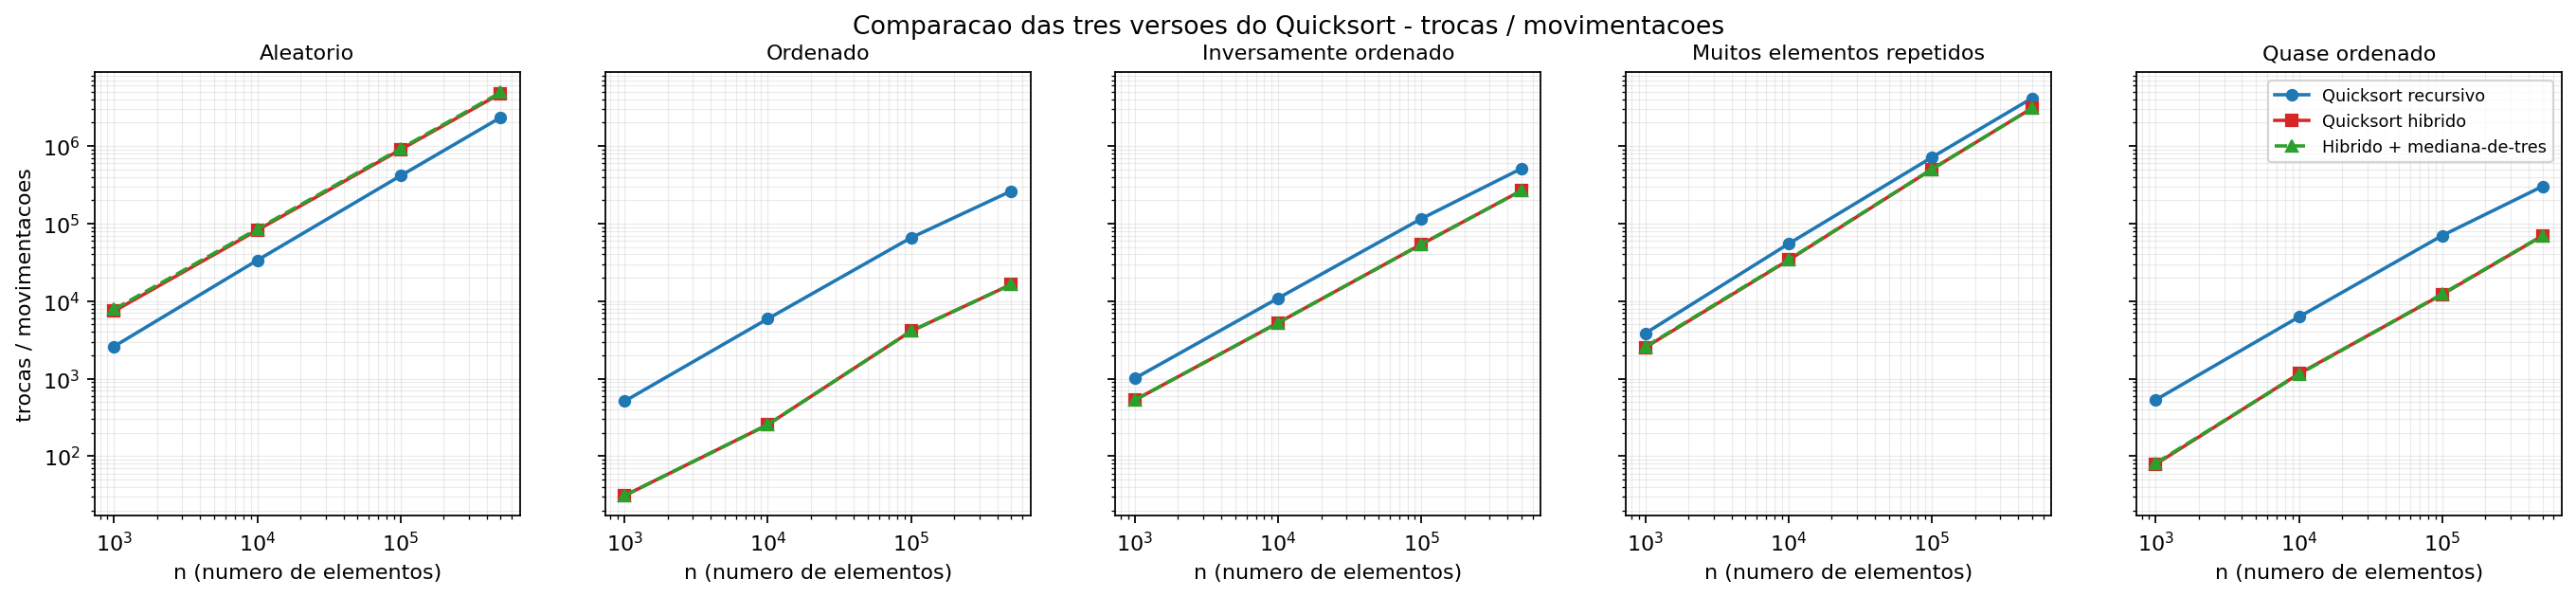
\includegraphics[width=\textwidth]{imagem/principal_trocas.png}
\caption{Número médio de trocas (movimentações) das três versões, por massa de teste.}
\label{fig:princ-trocas}
\end{figure}
\FloatBarrier

\begin{table}[H]
\centering
\caption{Resultados para a massa Aleatório.}
\label{tab:aleatorio}
\begin{tabular}{lrrrr}
\hline
\textbf{Versão} & \textbf{$n$} & \textbf{Tempo (ms)} & \textbf{Comparações} & \textbf{Trocas} \\
\hline
Recursivo & 1.000 & 0,037 & 13.323 & 2.600 \\
Híbrido & 1.000 & 0,021 & 14.435 & 7.414 \\
Mediana-3 & 1.000 & 0,026 & 14.109 & 7.829 \\
\hline
Recursivo & 10.000 & 0,459 & 180.022 & 33.586 \\
Híbrido & 10.000 & 0,341 & 191.362 & 82.044 \\
Mediana-3 & 10.000 & 0,348 & 180.820 & 85.022 \\
\hline
Recursivo & 100.000 & 5,435 & 2.238.090 & 412.988 \\
Híbrido & 100.000 & 4,338 & 2.351.171 & 897.440 \\
Mediana-3 & 100.000 & 4,387 & 2.242.553 & 923.525 \\
\hline
Recursivo & 500.000 & 30,016 & 13.041.446 & 2.332.566 \\
Híbrido & 500.000 & 24,586 & 13.610.714 & 4.754.782 \\
Mediana-3 & 500.000 & 24,915 & 12.386.071 & 4.911.093 \\
\hline
\end{tabular}
\end{table}

\begin{table}[H]
\centering
\caption{Resultados para a massa Ordenado.}
\label{tab:ordenado}
\begin{tabular}{lrrrr}
\hline
\textbf{Versão} & \textbf{$n$} & \textbf{Tempo (ms)} & \textbf{Comparações} & \textbf{Trocas} \\
\hline
Recursivo & 1.000 & 0,005 & 9.009 & 511 \\
Híbrido & 1.000 & 0,003 & 5.942 & 31 \\
Mediana-3 & 1.000 & 0,003 & 6.004 & 31 \\
\hline
Recursivo & 10.000 & 0,064 & 125.439 & 5.904 \\
Híbrido & 10.000 & 0,041 & 89.497 & 255 \\
Mediana-3 & 10.000 & 0,041 & 90.007 & 255 \\
\hline
Recursivo & 100.000 & 0,805 & 1.600.016 & 65.535 \\
Híbrido & 100.000 & 0,562 & 1.291.821 & 4.095 \\
Mediana-3 & 100.000 & 0,559 & 1.300.011 & 4.095 \\
\hline
Recursivo & 500.000 & 4,104 & 9.000.018 & 262.143 \\
Híbrido & 500.000 & 3,141 & 7.467.247 & 16.383 \\
Mediana-3 & 500.000 & 3,132 & 7.500.013 & 16.383 \\
\hline
\end{tabular}
\end{table}

\begin{table}[H]
\centering
\caption{Resultados para a massa Inverso.}
\label{tab:inverso}
\begin{tabular}{lrrrr}
\hline
\textbf{Versão} & \textbf{$n$} & \textbf{Tempo (ms)} & \textbf{Comparações} & \textbf{Trocas} \\
\hline
Recursivo & 1.000 & 0,006 & 9.016 & 1.010 \\
Híbrido & 1.000 & 0,004 & 5.946 & 530 \\
Mediana-3 & 1.000 & 0,004 & 6.009 & 530 \\
\hline
Recursivo & 10.000 & 0,071 & 125.452 & 10.904 \\
Híbrido & 10.000 & 0,048 & 89.504 & 5.254 \\
Mediana-3 & 10.000 & 0,048 & 90.015 & 5.254 \\
\hline
Recursivo & 100.000 & 0,861 & 1.600.030 & 115.534 \\
Híbrido & 100.000 & 0,618 & 1.291.832 & 54.094 \\
Mediana-3 & 100.000 & 0,618 & 1.300.023 & 54.094 \\
\hline
Recursivo & 500.000 & 4,371 & 9.000.034 & 512.142 \\
Híbrido & 500.000 & 3,404 & 7.467.260 & 266.382 \\
Mediana-3 & 500.000 & 3,434 & 7.500.027 & 266.382 \\
\hline
\end{tabular}
\end{table}

\begin{table}[H]
\centering
\caption{Resultados para a massa Repetidos (10 chaves distintas).}
\label{tab:repetidos}
\begin{tabular}{lrrrr}
\hline
\textbf{Versão} & \textbf{$n$} & \textbf{Tempo (ms)} & \textbf{Comparações} & \textbf{Trocas} \\
\hline
Recursivo & 1.000 & 0,020 & 10.427 & 3.840 \\
Híbrido & 1.000 & 0,009 & 7.806 & 2.524 \\
Mediana-3 & 1.000 & 0,016 & 7.571 & 2.571 \\
\hline
Recursivo & 10.000 & 0,221 & 135.619 & 54.818 \\
Híbrido & 10.000 & 0,163 & 102.243 & 33.791 \\
Mediana-3 & 10.000 & 0,179 & 101.570 & 34.211 \\
\hline
Recursivo & 100.000 & 2,467 & 1.687.013 & 712.530 \\
Híbrido & 100.000 & 2,011 & 1.357.196 & 500.738 \\
Mediana-3 & 100.000 & 2,004 & 1.353.863 & 501.874 \\
\hline
Recursivo & 500.000 & 13,117 & 9.776.488 & 4.131.089 \\
Híbrido & 500.000 & 10,825 & 8.124.660 & 3.068.952 \\
Mediana-3 & 500.000 & 11,023 & 7.880.701 & 3.070.614 \\
\hline
\end{tabular}
\end{table}

\begin{table}[H]
\centering
\caption{Resultados para a massa Quase ordenado.}
\label{tab:quaseordenado}
\begin{tabular}{lrrrr}
\hline
\textbf{Versão} & \textbf{$n$} & \textbf{Tempo (ms)} & \textbf{Comparações} & \textbf{Trocas} \\
\hline
Recursivo & 1.000 & 0,006 & 9.030 & 533 \\
Híbrido & 1.000 & 0,004 & 5.989 & 79 \\
Mediana-3 & 1.000 & 0,004 & 6.112 & 81 \\
\hline
Recursivo & 10.000 & 0,072 & 125.767 & 6.252 \\
Híbrido & 10.000 & 0,048 & 90.778 & 1.159 \\
Mediana-3 & 10.000 & 0,048 & 91.981 & 1.140 \\
\hline
Recursivo & 100.000 & 0,904 & 1.607.418 & 70.047 \\
Híbrido & 100.000 & 0,650 & 1.302.115 & 12.210 \\
Mediana-3 & 100.000 & 0,651 & 1.316.461 & 12.367 \\
\hline
Recursivo & 500.000 & 4,698 & 9.043.946 & 300.847 \\
Híbrido & 500.000 & 3,668 & 7.527.613 & 69.366 \\
Mediana-3 & 500.000 & 3,688 & 7.599.189 & 69.628 \\
\hline
\end{tabular}
\end{table}

\subsection{Ganho das versões híbridas}

A Figura \ref{fig:ganho} apresenta a redução percentual de tempo das versões
híbridas em relação ao Quicksort recursivo puro.

\begin{figure}[H]
\centering
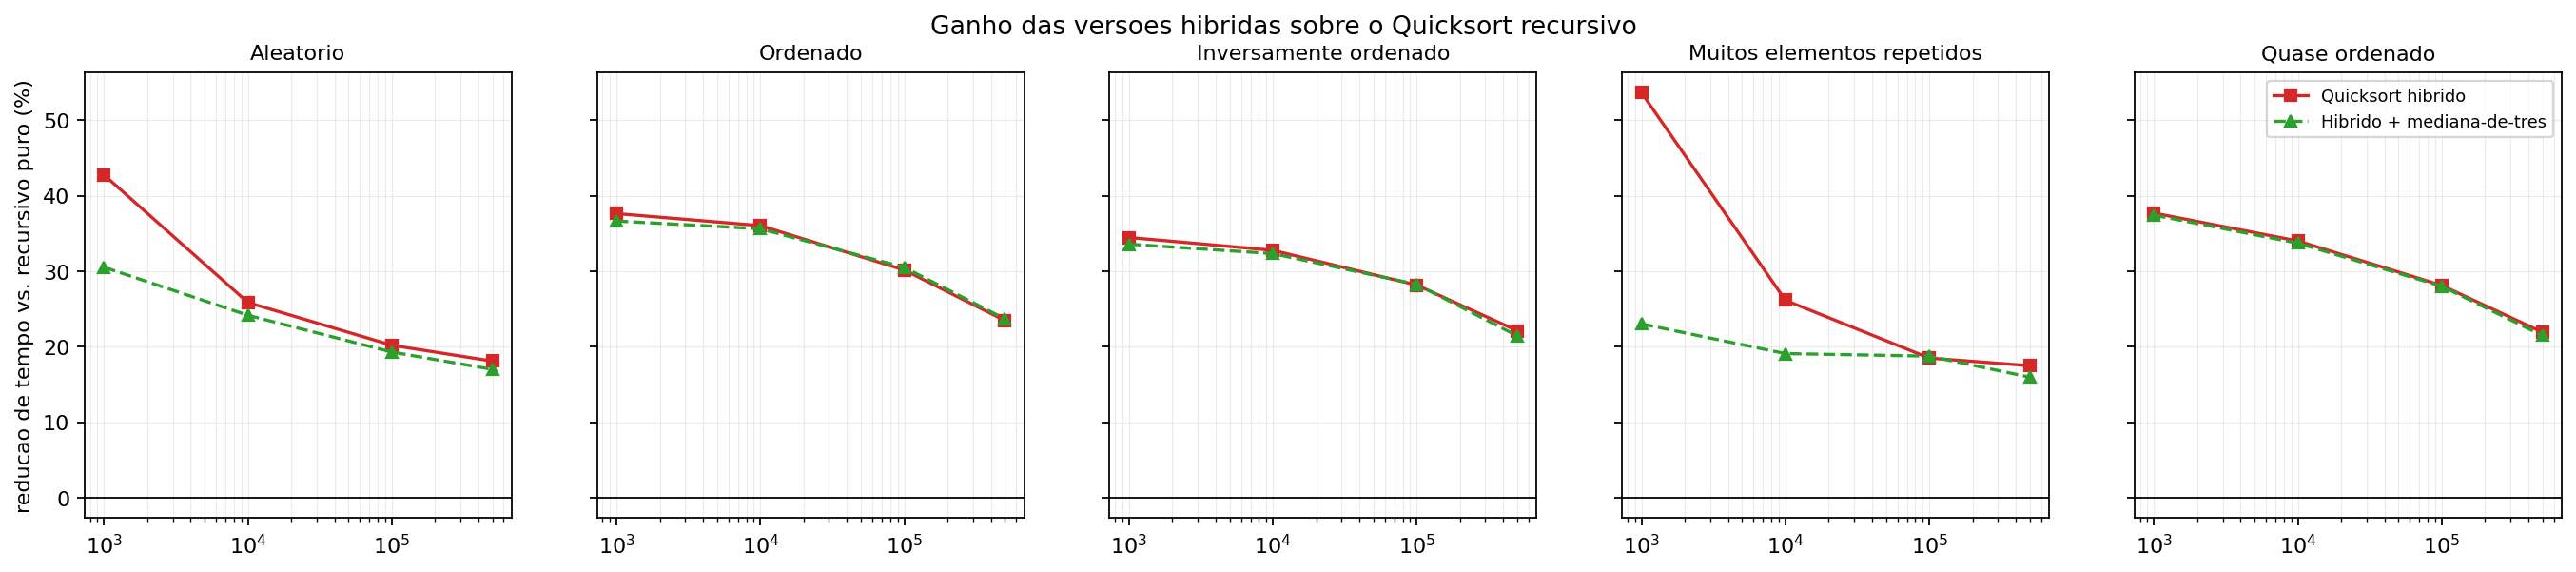
\includegraphics[width=0.95\textwidth]{imagem/ganho_relativo.png}
\caption{Redução do tempo de execução das versões híbridas em relação ao Quicksort recursivo.}
\label{fig:ganho}
\end{figure}
\FloatBarrier

O ganho é consistente: a redução de tempo varia entre \textbf{16\% e 54\%}, com
mediana de \textbf{28\%}, sem que nenhuma configuração apresente prejuízo. Confirma-se,
portanto, a hipótese que fundamenta a versão híbrida.

Cabe observar que o ganho é maior nas massas com estrutura (Ordenado, Quase
ordenado) do que na massa Aleatório. A razão é a adaptatividade do Insertion Sort
discutida na Seção \ref{sec:insertion}: em subvetores quase ordenados, o número de
deslocamentos é proporcional ao número de inversões, que é pequeno. Isso é visível na
Tabela \ref{tab:ordenado}, em que o número de trocas cai de 262.143 para 16.383 em
$n = 500.000$ --- redução de dezesseis vezes.

\subsection{Efeito da mediana-de-três}
\label{sec:efeito-mediana}

A comparação entre as versões (b) e (c) exige cautela metodológica. Confrontar a
versão com mediana-de-três ($M = 40$) diretamente com o Quicksort recursivo puro
($M = 1$) faria variar \textbf{duas} grandezas simultaneamente --- o corte $M$ e a
estratégia de pivô --- e atribuiria à mediana-de-três um ganho que decorre, em sua
maior parte, do corte. Para isolar o efeito do pivô, as duas versões devem ser
comparadas com o \textbf{mesmo valor de $M$}, conforme a Tabela \ref{tab:mediana3}.

\begin{table}[H]
\centering
\caption{Redução do número de comparações da mediana-de-três em relação ao híbrido simples, ambos com $M = 40$.}
\label{tab:mediana3}
\begin{tabular}{lrrrr}
\hline
\textbf{Massa} & \textbf{$n$=1.000} & \textbf{$n$=10.000} & \textbf{$n$=100.000} & \textbf{$n$=500.000} \\
\hline
Aleatório & $+2{,}26\%$ & $+5{,}51\%$ & $+4{,}62\%$ & $+9{,}00\%$ \\
Repetidos & $+3{,}01\%$ & $+0{,}66\%$ & $+0{,}25\%$ & $+3{,}00\%$ \\
Ordenado & $-1{,}04\%$ & $-0{,}57\%$ & $-0{,}63\%$ & $-0{,}44\%$ \\
Inverso & $-1{,}06\%$ & $-0{,}57\%$ & $-0{,}63\%$ & $-0{,}44\%$ \\
Quase ordenado & $-2{,}05\%$ & $-1{,}33\%$ & $-1{,}10\%$ & $-0{,}95\%$ \\
\hline
\multicolumn{5}{l}{\footnotesize Valores positivos indicam vantagem da mediana-de-três.} \\
\end{tabular}
\end{table}

A Figura \ref{fig:diferenca-mediana3} apresenta a mesma comparação de forma visual,
agora incluindo também o tempo, de modo que o efeito isolado do pivô (com $M$
constante) fica explícito.

\begin{figure}[H]
\centering
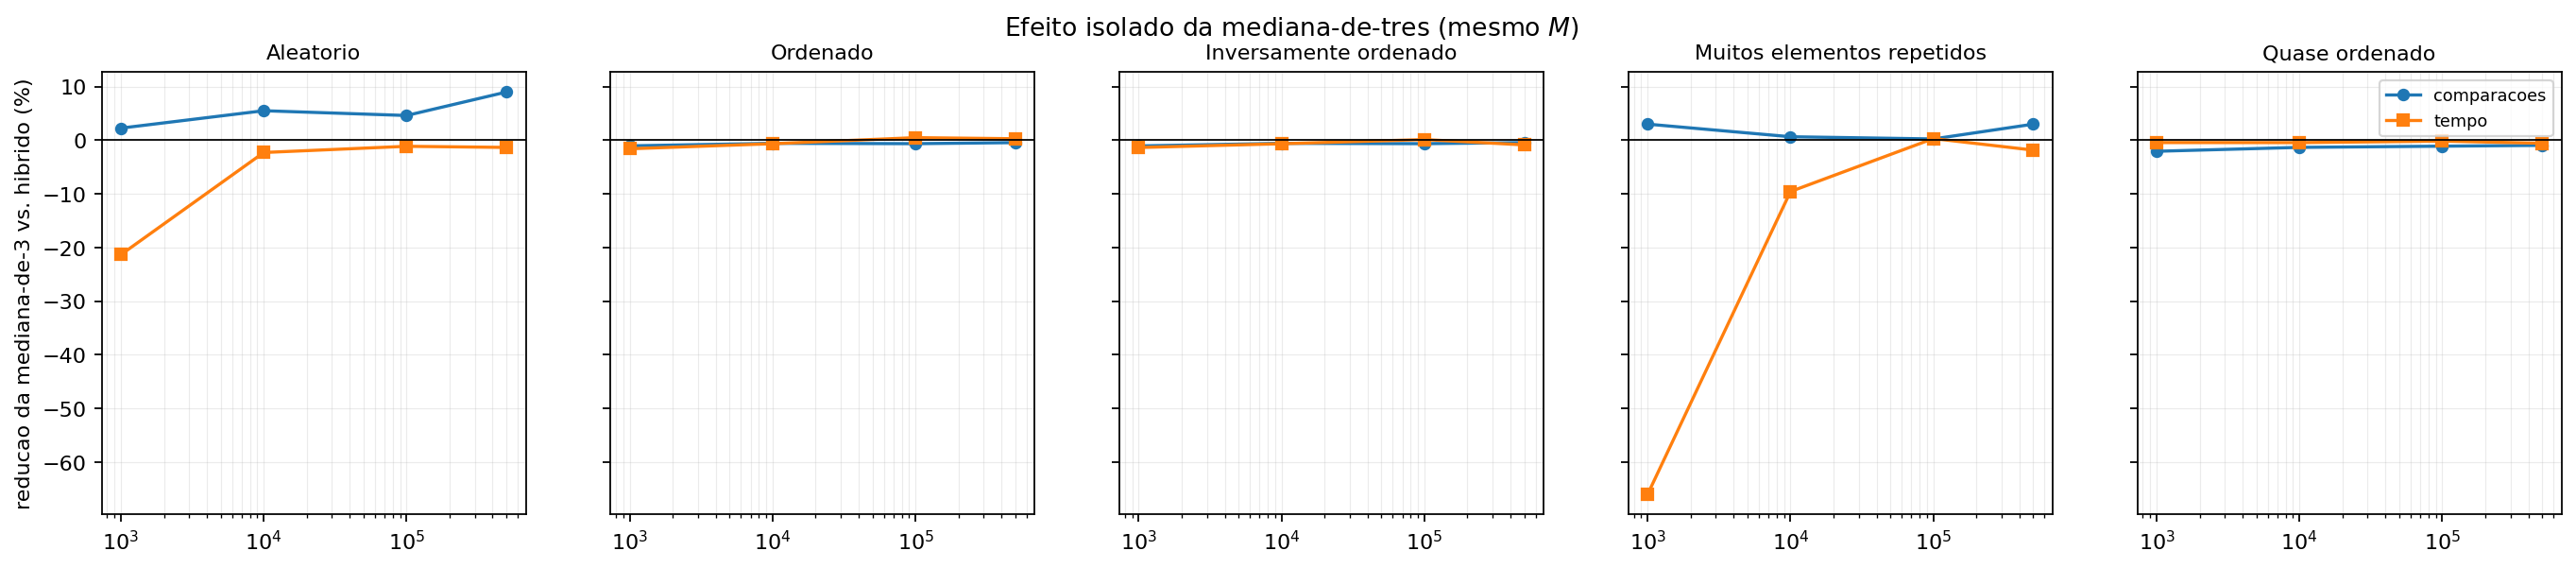
\includegraphics[width=\textwidth]{imagem/diferenca_mediana3.png}
\caption{Efeito isolado da mediana-de-três, ambos com $M = 40$: redução percentual das comparações e do tempo em relação ao híbrido simples. Valores positivos indicam vantagem da mediana-de-três.}
\label{fig:diferenca-mediana3}
\end{figure}
\FloatBarrier

O resultado é nítido e inteiramente explicado pela teoria:

\begin{itemize}
  \item Na massa \textbf{Aleatório}, a mediana-de-três reduz as comparações em 2\% a
        9\%. O elemento central de um vetor aleatório é um elemento qualquer da
        distribuição; a mediana de três amostras é um estimador melhor da mediana
        verdadeira do subvetor, produzindo partições mais equilibradas. A magnitude
        observada é compatível com a redução teórica de aproximadamente 14\% prevista
        por \citeonline{sedgewick1978} --- a diferença decorre de o corte em $M = 40$
        já eliminar as chamadas recursivas mais profundas, que são justamente aquelas
        em que o desbalanceamento mais pesa;

  \item Nas massas \textbf{Ordenado}, \textbf{Inverso} e \textbf{Quase ordenado}, a
        mediana-de-três é aproximadamente 1\% \textbf{pior}. A explicação é direta:
        em um vetor ordenado, o elemento central \textit{já é} a mediana exata do
        subvetor. A mediana-de-três seleciona exatamente o mesmo pivô, produzindo
        partições idênticas --- o que se confirma pelo número de trocas rigorosamente
        igual nas Tabelas \ref{tab:ordenado} e \ref{tab:inverso} --- e gasta, além
        disso, duas a três comparações adicionais por chamada.
\end{itemize}

Conclui-se que, quando comparada a um pivô central, \textbf{a mediana-de-três não
apresenta vantagem sistemática}. Seu valor real manifesta-se na comparação com pivôs
de \textbf{posição fixa}, como se demonstra na seção seguinte.

\section{Pior caso forçado}
\label{sec:res-piorcaso}

Para forçar explicitamente o pior caso, combinou-se \textbf{vetor já ordenado} com
\textbf{escolha inadequada de pivô} (primeiro elemento), conforme discutido na Seção
\ref{sec:piorcaso}. A Tabela \ref{tab:piorcaso} e a Figura \ref{fig:piorcaso}
apresentam os resultados.

\begin{table}[H]
\centering
\caption{Pior caso forçado: vetor ordenado com pivô igual ao primeiro elemento.}
\label{tab:piorcaso}
\begin{tabular}{lrrrr}
\hline
\textbf{Versão} & \textbf{$n$} & \textbf{Tempo (ms)} & \textbf{Comparações} & \textbf{Comp./$n^2$} \\
\hline
Pivô = primeiro & 1.000 & 0,138 & 501.498 & 0,5015 \\
Pivô = primeiro & 5.000 & 3,172 & 12.507.498 & 0,5003 \\
Pivô = primeiro & 10.000 & 12,679 & 50.014.998 & 0,5001 \\
Pivô = primeiro & 20.000 & 50,657 & 200.029.998 & 0,5001 \\
Pivô = primeiro & 50.000 & 309,115 & 1.250.074.998 & 0,5000 \\
\hline
Recursivo (central) & 50.000 & 0,378 & 750.015 & 0,0003 \\
Mediana-3 & 50.000 & 0,261 & 600.010 & 0,0002 \\
\hline
\end{tabular}
\end{table}

\begin{figure}[H]
\centering
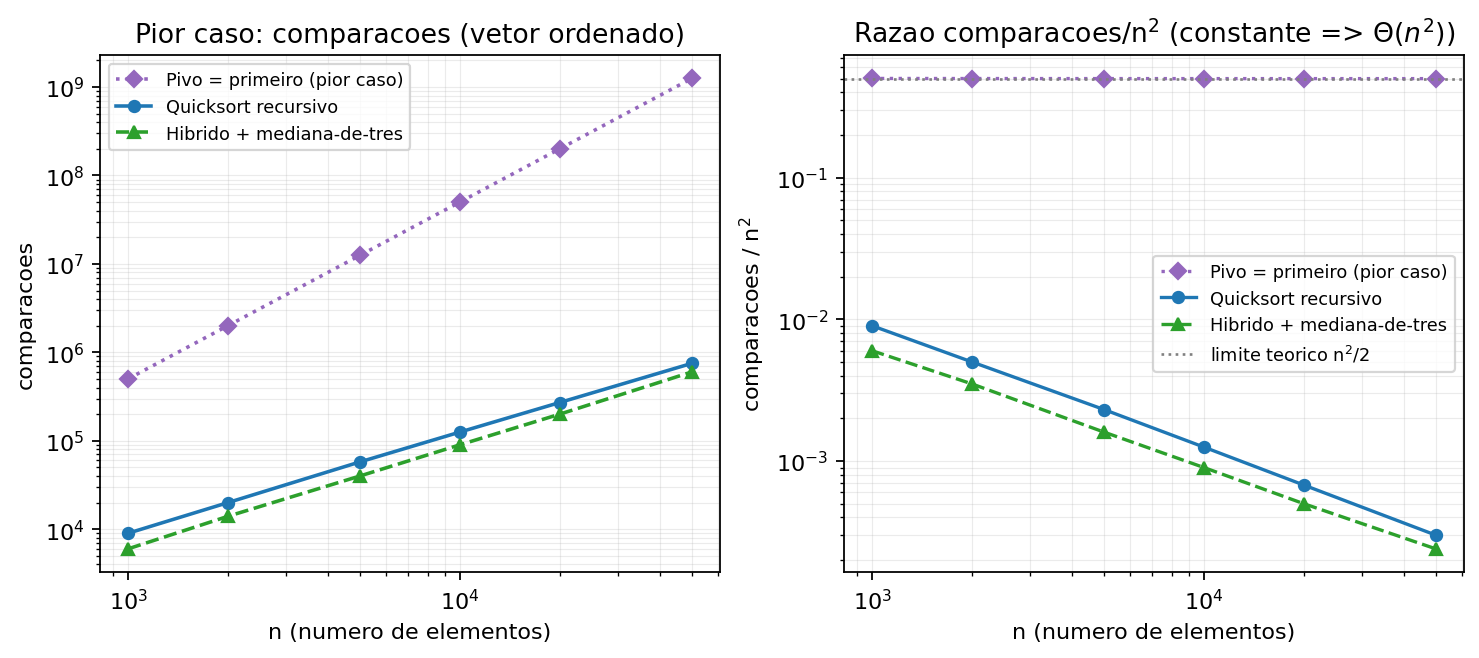
\includegraphics[width=\textwidth]{imagem/pior_caso.png}
\caption{Pior caso: número de comparações e razão comparações/$n^2$.}
\label{fig:piorcaso}
\end{figure}
\FloatBarrier

A razão comparações/$n^2$ converge para \textbf{exatamente $0{,}5000$}, confirmando
numericamente a previsão teórica da Equação \ref{eq:piorcaso}, segundo a qual o pior
caso executa $n(n-1)/2 \approx n^2/2$ comparações. O painel direito da Figura
\ref{fig:piorcaso} torna essa constatação visual: a curva do pivô inadequado é
horizontal, sobreposta ao limite teórico, enquanto as curvas das demais versões
decrescem --- comportamento esperado de funções $\Theta(n \log n)$, cuja razão sobre
$n^2$ tende a zero.

Em números absolutos, para $n = 50.000$ a versão com pivô inadequado executa
1.250.074.998 comparações contra 600.010 da versão com mediana-de-três: uma diferença
de aproximadamente \textbf{2.000 vezes}, refletida em tempo de execução
\textbf{1.200 vezes} maior (309,1 ms contra 0,261 ms).

Cabe registrar uma consequência prática frequentemente esquecida. No pior caso, a
profundidade da recursão é $n$, e não $O(\log n)$. Com a pilha padrão de 8 MB do
sistema utilizado, entradas superiores a aproximadamente 100.000 elementos
provocariam estouro de pilha --- motivo pelo qual este experimento foi limitado a
$n = 50.000$. Trata-se de uma falha de natureza distinta da lentidão: o programa não
apenas demora, ele termina anormalmente. Essa observação reforça o argumento de
\citeonline{musser1997} em favor do monitoramento da profundidade de recursão.

\section{Análise crítica}
\label{sec:analise-critica}

Dois resultados deste trabalho merecem análise mais detida, por contrariarem a
intuição derivada exclusivamente da análise assintótica.

\subsection{Mais comparações, menos tempo}

Observe-se a massa Aleatório na Tabela \ref{tab:aleatorio}. Para $n = 100.000$, o
Quicksort recursivo executa 2.238.090 comparações em 5,435 ms, enquanto a versão
híbrida executa 2.351.171 comparações --- \textbf{5\% a mais} --- em 4,338 ms,
sendo, portanto, \textbf{20\% mais rápida}. O mesmo padrão repete-se em todos os
tamanhos, e também no número de trocas, que mais que dobra na versão híbrida.

À primeira vista, o resultado é paradoxal: como pode um algoritmo que realiza mais
operações elementares ser mais rápido? A explicação está no fato de que
\textbf{nem toda operação elementar custa o mesmo}:

\begin{enumerate}
  \item \textbf{Custo por chamada recursiva.} Com $M = 1$, o Quicksort realiza
        aproximadamente $n$ chamadas recursivas, cada uma com prólogo, epílogo,
        manipulação de pilha e cálculo de pivô. Com $M = 40$, esse número cai
        cerca de 40 vezes. As comparações economizadas na recursão são substituídas
        por comparações do Insertion Sort, que não têm esse custo fixo associado;

  \item \textbf{Localidade de referência.} O Insertion Sort opera sobre blocos
        contíguos de no máximo 40 elementos --- 160 bytes, que cabem em três linhas de
        cache. Todos os acessos ocorrem em cache L1. Já as chamadas recursivas
        profundas do Quicksort tocam regiões dispersas do vetor;

  \item \textbf{Predição de desvios.} O laço do Insertion Sort tem padrão de desvio
        altamente previsível, ao passo que o desvio da partição do Quicksort depende
        da comparação com o pivô e é, por construção, imprevisível --- cada erro de
        predição custa entre 15 e 20 ciclos de \textit{pipeline}.
\end{enumerate}

Esse achado é coerente com a literatura recente discutida no Capítulo
\ref{cap:referencial}: \citeonline{kushagra2014} atribuem os ganhos do Quicksort de
múltiplos pivôs à redução de falhas de cache, e não à contagem de comparações, e
\citeonline{edelkamp2019} obtêm ganhos expressivos atuando exclusivamente sobre a
predição de desvios, sem alterar o número de comparações. A conclusão é que
\textbf{a contagem de comparações, isoladamente, deixou de ser um preditor confiável
do tempo de execução em hardware moderno} --- embora permaneça a métrica correta
para caracterizar a complexidade assintótica.

\subsection{O papel das métricas determinísticas}

O segundo resultado é de natureza metodológica. Como relatado na Seção
\ref{sec:medicao}, a primeira calibração de $M$ produziu um valor incorreto por
contaminação da medição de tempo pelo governador de frequência do processador.

O erro foi detectado porque \textbf{duas métricas mediam o mesmo fenômeno com
naturezas distintas}: o número de comparações é determinístico e reprodutível bit a
bit, enquanto o tempo é uma grandeza ruidosa. Quando as duas discordaram
sistematicamente, a métrica determinística evidenciou a existência de um problema na
medição.

Esse é, precisamente, o motivo pelo qual o enunciado exige a manutenção de contadores
de comparações e trocas \textbf{além} da medição de tempo. Os contadores não são
apenas uma métrica complementar de desempenho: funcionam como instrumento de
verificação da própria medição experimental. Sem eles, o valor incorreto de $M$
teria sido incorporado a este relatório sem qualquer sintoma perceptível.
